\subsection{Khái niệm}
Là quá trình tính toán để tìm ra các mẫu trong các bộ dữ liệu lớn liên quan đến các phương pháp tại giao điểm của máy học, thống kê và các hệ thống cơ sở dữ liệu. 
Đây là một lĩnh vực liên ngành của khoa học máy tính. Mục tiêu tổng thể của quá trình khai thác dữ liệu là trích xuất thông tin từ một bộ dữ liệu và chuyển nó thành một cấu trúc dễ hiểu để sử dụng tiếp. 
Ngoài bước phân tích thô, nó còn liên quan tới cơ sở dữ liệu và các khía cạnh quản lý dữ liệu, xử lý dữ liệu trước, suy xét mô hình và suy luận thống kê, các thước đo thú vị, các cân nhắc phức tạp, xuất kết quả về các cấu trúc được phát hiện, hiện hình hóa và cập nhật trực tuyến.
\subsection{Các bước trong quá trình khai phá}
Quá trình được thực hiện qua 9 bước:
\begin{enumerate}
    \item \textbf{Tìm hiểu lĩnh vực của bài toán (ứng dụng)}: Các mục đích của bài toán,
    các tri thức cụ thể của lĩnh vực.
    \item \textbf{Tạo nên (thu thập) một tập dữ liệu phù hợp.}
    \item \textbf{Làm sạch và tiền xử lý dữ liệu.}
    \item \textbf{Giảm kích thức của dữ liệu, chuyển đổi dữ liệu}: Xác định thuộc tính quan
    trọng, giảm số chiều (số thuộc tính), biểu diễn bất biến.
    \item \textbf{Lựa chọn chức năng khai phá dữ liệu}: Phân loại, gom cụm, dự báo, sinh
    ra các luật kết hợp.
    \item \textbf{Lựa chọn/ Phát triển (các) giải thuật khai phá dữ liệu phù hợp.}
    \item \textbf{Tiến hành khai phá dữ liệu.}
    \item \textbf{Đánh giá mẫu thu được và biểu diễn tri thức}: Hiển thị hóa, chuyển đổi, bỏ
    đi các mẫu dư thừa,…
    \item \textbf{Sử dụng tri thức được khai phá.}
\end{enumerate}
Quá trình khám phá tri thức theo cách nhìn của giới nghiên cứu về các hệ
thống dữ liệu và kho dữ liệu về quá trình khám phá tri thức
\begin{itemize}
    \item Chuẩn bị dữ liệu \textit{(data preparation)}, bao gồm các quá trình làm sạch dữ liệu
    \textit{(data cleaning)}, tích hợp dữ liệu \textit{(data integration)}, chọn dữ liệu \textit{(data selection)},
    biến đổi dữ liệu \textit{(data transformation)}.
    \item Khai thác dữ liệu \textit{(data mining)}: xác định nhiệm vụ khai thác dữ liệu và lựa
    chọn kỹ thuật khai thác dữ liệu. Kết quả cho ta một nguồn tri thức thô.
    \item Đánh giá \textit{(evaluation)}: dựa trên một số tiêu chí tiến hành kiểm tra và lọc
    nguồn tri thức thu được. 
    \item Triển khai \textit{(deployment)}.
    \item Quá trình khai thác tri thức không chỉ là một quá trình tuần tự từ bước đầu
    tiên đến bước cuối cùng mà là một quá trình lặp và có quay trở lại các bước đã qua.
\end{itemize}
\begin{figure}[!htbp]
    \centering
    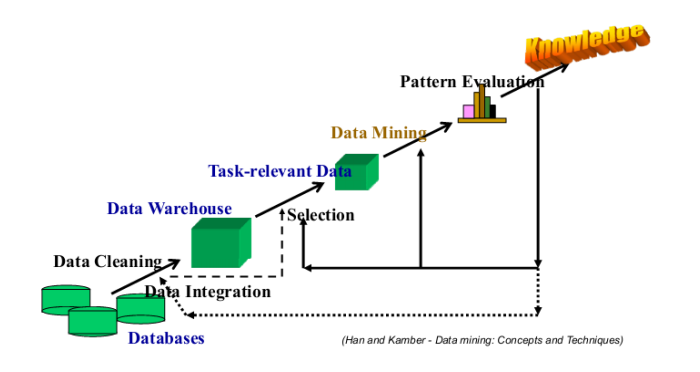
\includegraphics[scale=0.7]{data_mining}
    \caption{Quá trình khai phá tri thức}
    \label{fig:x cubed graph}
\end{figure}
\FloatBarrier
\subsection{Ứng dụng của khai phá dữ liệu}
\begin{itemize}
    \item Kinh tế - ứng dụng trong kinh doanh, tài chính, tiếp thị bán hàng, bảo hiểm,
    thương mại, ngân hàng, … Đưa ra các bản báo cáo giàu thông tin; phân tích rủi ro
    trước khi đưa ra các chiến lược kinh doanh, sản xuất; phân loại khách hàng từ đó phân định thị trường, thị phần; …
    \item Khoa học: Thiên văn học – dự đoán đường đi các thiên thể, hành tinh, …;
    Công nghệ sinh học – tìm ra các gen mới, cây con giống mới, …; …
    \item Web: các công cụ tìm kiếm.  
\end{itemize}